\chapter{Introduction}
\label{chap:introduction}

QMCPACK is an open-source, high-performance electronic structure code that implements numerous Quantum Monte Carlo algorithms.

Test of the bibliography\cite{CeperleyAlderPRL1980}.

\section{Quickstart and a first QMCPACK calculation}
If you are keen to get started this section describes how to quickly
build and run QMCPACK on standard UNIX or Linux-like system. The
autoconfiguring build system often works directly on these
systems. For a standard
Linux system where C++, MPI, BLAS/LAPACK, FFTW, HDF5, and CMake are already installed,
QMCPACK can be built and run within five minutes. For supercomputers, cross-compilation systems, and other computer
clusters the build system may require hints on the locations of
libraries and which versions to use,  see Chapter
\ref{chap:obtaininginstalling}.

To build QMCPACK:

\begin{enumerate}
\item Download the latest QMCPACK distribution from
  \url{http://www.qmcpack.org}
\item Untar the archive, e.g., \texttt{tar xvf
    qmcpack\_revNNNN\_YYYYMMDD.tar.gz}
\item Run CMake in a suitable build directory to configure QMCPACK for
  your system: \texttt{cd
    qmcpack/build; cmake ..}
\item If CMake is unable to find all needed libraries, see Chapter
  \ref{chap:obtaininginstalling} for instructions and specific build
  instructions for common systems.
\item Build QMCPACK: \texttt{make} or \texttt{make -j 24}, the latter
  for a faster parallel build on a system using, e.g., up to 24 processes.
\item The QMCPACK executable is \texttt{bin/qmcapp}
\end{enumerate}

QMCPACK is distributed with examples illustrating different
capabilities. Most of the examples are designed to run quickly with
modest resources. We'll run a short diffusion Monte Carlo calculation
of a water molecule:

\begin{enumerate}
\item Go to the appropriate example directory: \texttt{cd
    ../examples/molecules}
\item (Optional) Put the QMCPACK binary on your path:\\ \texttt{export PATH=\$PATH:location-of-qmcpack/build/bin}
\item Run QMCPACK: \texttt{../../build/bin/qmcapp simple-H2O.xml} or
  \texttt{qmcapp simple-H2O.xml} if you followed the step above.
\item The run will output to the screen and generate a number of files:
\begin{verbatim}
$ls H2O*
H2O.HF.wfs.xml      H2O.s001.scalar.dat H2O.s002.cont.xml   H2O.s002.qmc.xml    H2O.s002.stat.h5
H2O.s001.qmc.xml    H2O.s001.stat.h5    H2O.s002.dmc.dat    H2O.s002.scalar.dat
\end{verbatim}
\item The results are in files with suffixes scalar.dat and dmc.dat . They are viewable with any standard editor.
\end{enumerate}

If you have python with matplotlib installed, you can use the
\texttt{qmca} analysis utility to produce statistics and plots of the
data. See Chapter \ref{chap:analysing} for information on analysing
QMCPACK data.
\begin{verbatim}
export PATH=$PATH:location-of-qmcpack/nexus/executables 
export PYTHONPATH=$PYTHONPATH:location-of-qmcpack/nexus/library
qmca H2O.s002.scalar.dat         # For statistical analysis of the DMC data
qmca -t -q e H2O.s002.scalar.dat # Graphical plot of DMC energy
\end{verbatim}

The last command should produce a graph as per
Fig. \ref{fig:quick_qmca_dmc_trace}. This shows the average energy of
the DMC walkers at each timestep. In a real simulation we would have
to check equilibration, convergence with walker population, timestep etc.

Congratulations, you have completed a DMC calculation with QMCPACK!

\begin{figure}
  \centering
  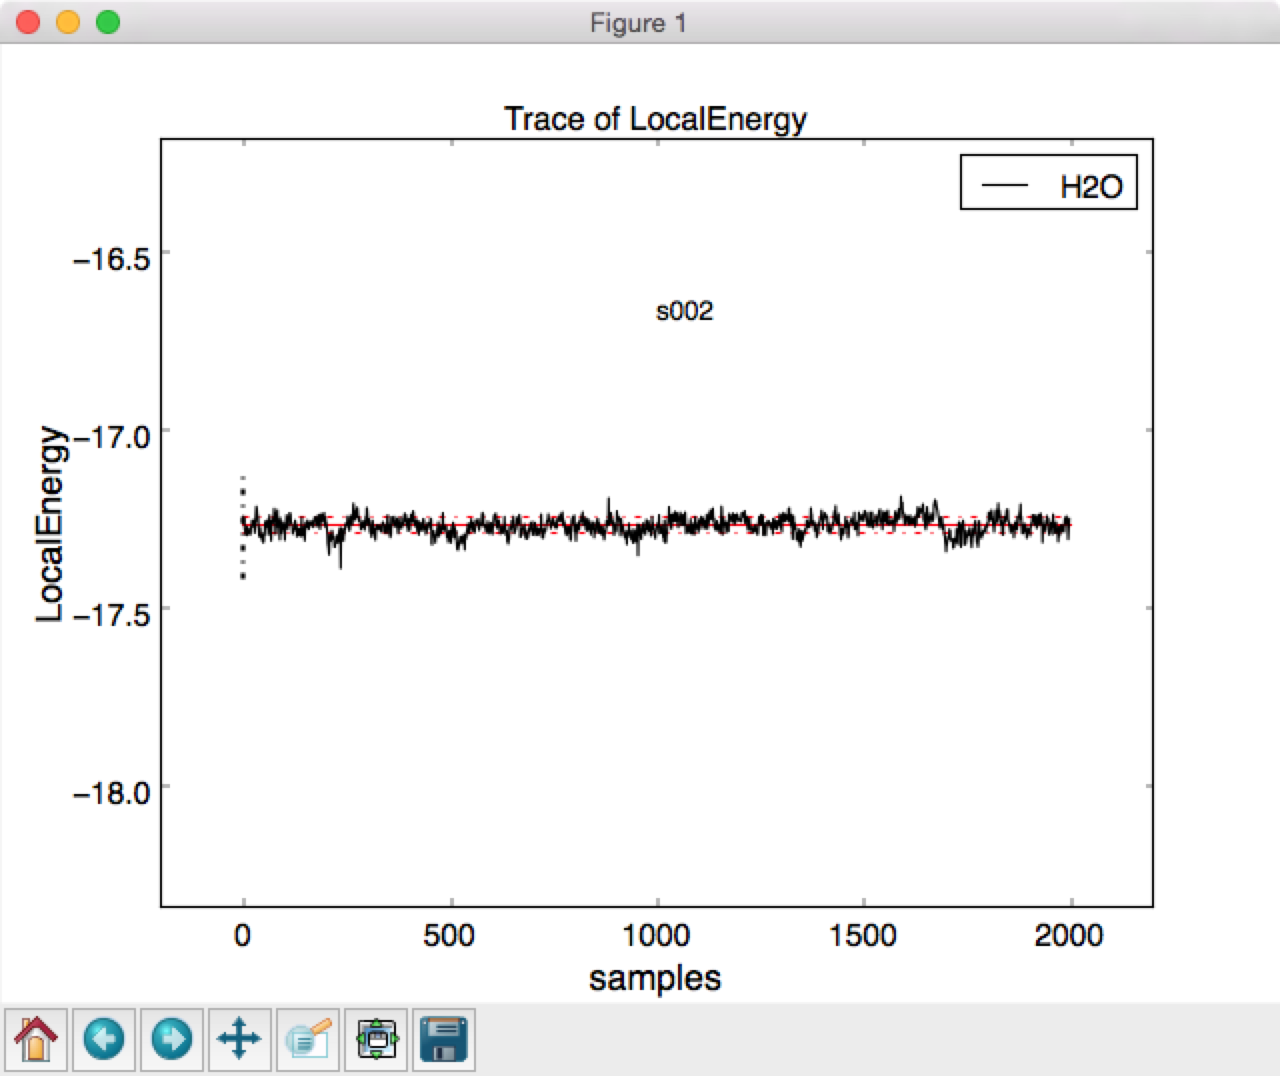
\includegraphics[width=10cm]{figures/quick_qmca_dmc_trace.png}
  \caption{Trace of walker energies produced by qmca tool for simple
    water molecule example.}
  \label{fig:quick_qmca_dmc_trace}
\end{figure}

\section{Authors and History}
\label{sec:history}
QMCPACK was initially written by Jeongnim Kim while in the group of
Prof. David Ceperley at the University of Illinois at
Urbana-Champaign, with later contributations at Oak Ridge National Laboratory. Over the years, many others have contributed, particularly
students and researchers in the groups of Prof. David Ceperley
and Prof. Richard M. Martin, as well as staff at Lawrence Livermore
National Laboratory, Sandia National Laboratories, Argonne National
Laboratory, and Oak Ridge National Laboratory.

The primary and original author of the code is Jeongnim
Kim. Developers, contributors, and advisors include:

Anouar Benali,  
David M. Ceperley, 
Simone Chiesa,
Raymond C. III Clay,
Chris Delaney,
Kenneth P. Esler,
Jaron T. Krogel,
Ying Wai Li,
Ye Luo,
Jeremy McMinis,
Miguel Morales,
William D. Parker,
Nichols A. Romero,
Luke Shulenburger,
Norman M. Tubman,
Jordan E. Vincent,
\ldots

Please let us know if you wish to be listed!

Development of QMCPACK has been supported by:
\begin{itemize}
\item “Network for ab initio many-body methods: development, education
  and training“ supported through the Predictive
  Theory and Modeling for Materials and Chemical Science program by
  the U.S. Department of Energy Office of Science, Basic Energy
  Sciences.
\item QMC Endstation, supported by Accelerating Delivery of Petascale
  Computing Environment At the DOE Leadership Computing Facility at
  ORNL, DOE. 
\item PetaApps, supported by the U. S. National Science
  Foundation.
\item Materials Computational Center, supported by the
  U.S. National Science Foundation.
\end{itemize}



\section{Support}
\label{sec:support}

\section{Performance}
\label{sec:performance}

\section{Open source license}
\label{sec:license}

QMCPACK is distributed under the University of Illinois/NCSA Open
Source License. 

\begin{verbatim}
		  University of Illinois/NCSA Open Source License

Copyright (c) 2003, University of Illinois Board of Trustees.
All rights reserved.

Developed by:   
  Jeongnim Kim
  Condensed Matter Physics,
  National Center for Supercomputing Applications, University of Illinois
  Materials computation Center, University of Illinois
  http://www.mcc.uiuc.edu/qmc/

Permission is hereby granted, free of charge, to any person obtaining a
copy of this software and associated documentation files (the
``Software''), to deal with the Software without restriction, including
without limitation the rights to use, copy, modify, merge, publish,
distribute, sublicense, and/or sell copies of the Software, and to
permit persons to whom the Software is furnished to do so, subject to
the following conditions:

        * Redistributions of source code must retain the above copyright 
          notice, this list of conditions and the following disclaimers.
        * Redistributions in binary form must reproduce the above copyright 
          notice, this list of conditions and the following disclaimers in 
          the documentation and/or other materials provided with the 
          distribution.
        * Neither the names of the NCSA, the MCC, the University of Illinois, 
          nor the names of its contributors may be used to endorse or promote 
          products derived from this Software without specific prior written 
          permission.

THE SOFTWARE IS PROVIDED "AS IS", WITHOUT WARRANTY OF ANY KIND, EXPRESS
OR IMPLIED, INCLUDING BUT NOT LIMITED TO THE WARRANTIES OF MERCHANTABILITY, 
FITNESS FOR A PARTICULAR PURPOSE AND NONINFRINGEMENT. IN NO EVENT SHALL 
THE CONTRIBUTORS OR COPYRIGHT HOLDERS BE LIABLE FOR ANY CLAIM, DAMAGES OR 
OTHER LIABILITY, WHETHER IN AN ACTION OF CONTRACT, TORT OR OTHERWISE, 
ARISING FROM, OUT OF OR IN CONNECTION WITH THE SOFTWARE OR THE USE OR 
OTHER DEALINGS WITH THE SOFTWARE.

\end{verbatim}

\section{Contributing to QMCPACK}
\label{sec:contributing}

\section{Roadmap}
\label{sec:roadmap}

\subsection{Documentation}

\subsection{QMCPACK}
